\documentclass{article}
\usepackage[margin=1in]{geometry}
\usepackage{amsmath,amsthm,amssymb}
\usepackage{bbm,enumerate,mathtools}
\usepackage{tikz,pgfplots}
\usepackage{chessboard}
\usepackage[hidelinks]{hyperref}
\usepackage{multicol} % Problem 35
\usepackage{xstring} % Difficulty command
\usetikzlibrary{shapes.geometric}

\newenvironment{question}{\begin{trivlist}\item[\textbf{Question.}]}{\end{trivlist}}
\newenvironment{note}{\begin{trivlist}\item[\textbf{Note.}]}{\end{trivlist}}
\newenvironment{references}{\begin{trivlist}\item[\textbf{References.}]}{\end{trivlist}}
\newenvironment{related}{\begin{trivlist}\item[\textbf{Related.}]\end{trivlist}\begin{enumerate}}{\end{enumerate}}

\newcommand\score[1]{
\pgfmathsetmacro\pgfxa{#1+1}
\tikzstyle{scorestars}=[
  star,
  star points=5,
  star point ratio=2.25,
  draw,
  inner sep=3pt,
  anchor=outer point 5
]
  \begin{tikzpicture}[baseline]
    \draw[opacity=0] (0,-0.5) rectangle (0,0.2); % Workaround for whitespace at the bottom.
    \foreach \i in {1,...,4} {
      \pgfmathparse{(\i<=#1?"yellow":"gray")}
      \edef\starcolor{\pgfmathresult}
      \draw (\i*4.5ex,0) node[name=star\i,scorestars,fill=\starcolor]  {};
    }
  \end{tikzpicture}
}

\newcommand{\difficulty}[1]{%
  \IfEqCase{#1}{%
      {1}{
        
\begin{tikzpicture}[scale=0.7, baseline=0.9mm]%
          \definecolor{slopegreen}{rgb}{0.0, 0.5, 0.0}%
          \fill[slopegreen] (0.5,0.5) circle (0.5);%
        \end{tikzpicture}%
      }%
      {2}{
        
\begin{tikzpicture}[scale=0.7, baseline=0.9mm]%
          \definecolor{slopeblue}{rgb}{0.0, 0.44, 1.00}
          \fill[slopeblue] (0,0) rectangle (1,1);%
        \end{tikzpicture}%
      }%
      {3}{
\begin{tikzpicture}[scale=0.7, baseline=0.9mm]\fill (0,0.5)--(0.5, 0)--(1,0.5)--(0.5,1)--cycle; \end{tikzpicture}}%
      {4}{
\begin{tikzpicture}[scale=0.7, baseline=0.9mm]\fill (0.25,0)--(0,0.5)--(0.25,1)--(0.5,0.5)--cycle; \fill (0.75,0)--(0.5,0.5)--(0.75,1)--(1,0.5)--cycle;\end{tikzpicture}}%
      % you can add more cases here as desired
  }[\PackageError{difficulty}{Undefined difficulty level: #1}{}]%
}%
\newcommand{\rating}[2]{\difficulty{#1}\\\score{#2}\\}


\begin{document}
\rating{2}{2}
Consider all $r$-colorings of the $n \times m$ grid where no two colors
are adjancent (horizontally/vertically) more than once.

\begin{figure}[!h]
  \centering
  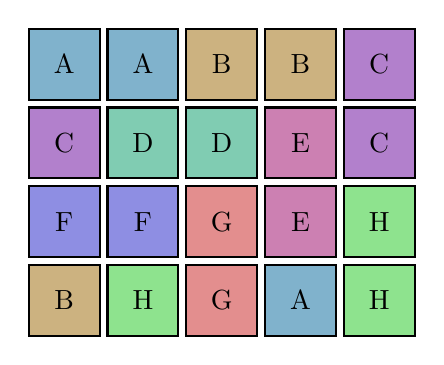
\begin{tikzpicture}
    \def\polyomino{
      0/3/0/2/3/5/A, 1/3/0/2/3/5/A, 2/3/3/2/0/5/B, 3/3/3/2/0/5/B, 4/3/2/0/3/5/C,
      0/2/2/0/3/5/C, 1/2/0/3/2/5/D, 2/2/0/3/2/5/D, 3/2/3/0/2/5/E, 4/2/2/0/3/5/C,
      0/1/1/1/7/9/F, 1/1/1/1/7/9/F, 2/1/7/1/1/9/G, 3/1/3/0/2/5/E, 4/1/1/7/1/9/H,
      0/0/3/2/0/5/B, 1/0/1/7/1/9/H, 2/0/7/1/1/9/G, 3/0/0/2/3/5/A, 4/0/1/7/1/9/H
    }
    %
    % [1, 1, 2, 2, 3]
    % [3, 4, 4, 5, 3]
    % [6, 6, 7, 5, 8]
    % [2, 8, 7, 1, 8]
    \foreach \x/\y/\r/\g/\b/\w/\l in \polyomino {
      \draw[thick,fill={rgb:red,\r;green,\g;blue,\b;white,\w}] (\x - 0.45, \y - 0.45) rectangle (\x + 0.45, \y + 0.45) node[pos=.5] {\l};
    }
  \end{tikzpicture}\\
  \caption{An $8$-coloring of the $4 \times 5$ grid where no two colors are adjancent
    more than once. There is no $7$-coloring.}
\end{figure}

\begin{question}
  Let $r_{n\times m}$ be the smallest integer such that there exists an
  $r_{n \times m}$-coloring of the $n \times m$ grid. What is $r_{n\times m}$?
\end{question}
\begin{related}
  \item What if colors are not allowed to be self-adjacent?
  \item How many $a(n, m)$-colorings exist up to permutation of the colors?
  \item What if this is done on a triangular or hexagonal grid?
  \item What if orientation matters?
    (A horizontal adjacency is distinct from a vertical adjacency.)
  \item What if order matters? (red-green is distinct from green-red.)
  \item What if diagonal adjacencies are considered?
\end{related}

\begin{note}
  \[
    \begin{array}{ccccc}
      r_{1 \times 1} = 1 \\
      r_{1 \times 2} = 1 & r_{2 \times 2} = 3 \\
      r_{1 \times 3} = 2 & r_{2 \times 3} = 4 & r_{3 \times 3} = 5 \\
      r_{1 \times 4} = 2 & r_{2 \times 4} = 5 & r_{3 \times 4} = 6 & r_{4 \times 4} = 7 \\
      r_{1 \times 5} = 3 & r_{2 \times 5} = 5 & r_{3 \times 5} = 7 & r_{4 \times 5} = 8 & r_{5 \times 5} = 9
    \end{array}
  \]
\end{note}

\begin{references}
  \item Problem 23.
  \item Problem 36.
  \item Problem 49.
\end{references}
\end{document}
